\documentclass[12pt,a4paper,UTF8]{article}
\usepackage{ctex} % Chinese support
\usepackage{graphicx} % Insert images
\usepackage{subfigure}
\usepackage{float}
\usepackage{listings} % Print source code
\usepackage{color} % Color support
\usepackage{booktabs} % Professional table support
\usepackage{pdflscape} % Landscape pages support in PDF
\usepackage{hyperref} % Hypertext links support for cross-referencing
\usepackage{amsmath,mathtools}
\usepackage{amssymb} % for ticks
\usepackage{ulem} % strikethrough

% Customize hyperref format (it's set to no special format here)
\hypersetup{hidelinks}

% Declare directories to search for graphics files for graphicx
\graphicspath{{figures/}}

% Define source code style for listings
\lstdefinestyle{verilog-style}{
	language=Verilog,
	basicstyle=\ttfamily\footnotesize,
	keywordstyle=\bfseries\color[rgb]{0, 0, 1},
	identifierstyle=\color[rgb]{0.5, 0.3, 0.1},
	stringstyle=\color[rgb]{0.6, 0.1, 0.1},
	commentstyle=\itshape\color[rgb]{0.05, 0.5, 0.05},
	backgroundcolor=\color[gray]{0.95},
	numbers=left,
	numbersep=5pt,
	numberstyle=\color[gray]{0.6},
  breaklines=true,
  escapeinside=``
}

\newcommand{\reporttitle}[2]{
  \LARGE\textsf{#1}\quad\underline{\makebox[12em]{#2}}
}

\newcommand{\reportinfo}[2]{
  \large\makebox[4em]{\textsf{#1}}\quad\underline{\makebox[18em]{#2}}
}

\begin{document}
\begin{titlepage}
  \centering
  \vspace*{\fill}
  {\Huge\textsf{数字电路与数字系统实验}} \\ [100pt]
  \reportinfo{实验名称}{exp07 存储器} \\ [10pt]
  \reportinfo{院系}{计算机科学与技术系} \\ [10pt]
  \reportinfo{学生姓名}{} \\ [10pt]
  \reportinfo{学号}{} \\ [10pt]
  \reportinfo{班级}{数字电路与数字系统实验1班} \\ [10pt]
  \reportinfo{邮箱}{} \\ [10pt]
  \reportinfo{实验时间}{2020 年 10 月 12 日} \\ [10pt]
  \vspace*{\fill}
\end{titlepage}
\tableofcontents
\newpage

\section{实验目的}
\begin{itemize}
  \item \sout{复习存储器} 上学期貌似只学过
        寄存器没学过存储器
  \item 学习用Verilog实现存储器
  \item 了解FPGA开发板上的存储器的特性
\end{itemize}

\section{实验原理}
将数据地址送入输入地址端或输出地址端,存储器根据
写使能信号读取相应地址对应数据,并进行写入或读出。

\section{实验环境/器材}
\begin{itemize}
  \item Quartus编辑器和DE10-Standard开发平台
  \item FPGA开发板
\end{itemize}

\section{程序代码+实验过程+测试方法}
\subsection{实验7.2 思考题}
该存储器的行为会发生变化。

连续赋值语句会把输出地址对应的数据立即输出。非阻塞赋值语句
会等到写使能无效的时候,再去取输出地址对应的数据,并输出。

例如当输入地址和输出地址为同一地址时,当写使能有效时,
连续赋值语句会把写入的数据立即送到输出总线上;非阻塞赋值语句
会等到写使能无效的时候,再取输出输出地址对应的数据。

也就是说,使用连续赋值语句,会让存储器的输出不受时钟
和使能端的控制。使用非阻塞赋值语句,会让存储器的输出
受时钟和使能端的控制。

\subsection{实验7.4 不同方式实现两个存储器}
先说明一下FPGA开发板上的按钮分配。因为要在一个工程里实现
两个存储器,所以用一个控制开关\mbox{KEY[1]}选择\mbox{RAM1}
(\mbox{KEY[1]=1})或者\mbox{RAM2}(\mbox{KEY[1]=0}),
并用一对LEDR来显示我们选择了哪个存储器。然后我们把
\mbox{KEY[0]}作为共用的写使能信号(按下为写使能有效)、
把\mbox{SW[9:8]}作为共用的数据输入、把\mbox{SW[7:4]}
作为共用的输入(写)地址、把\mbox{SW[3:0]}作为共用的输出(读)
地址。读数据时,我们把\mbox{RAM1}上的数据输出到\mbox{HEX1}和\linebreak[4]
\mbox{HEX0}上、把\mbox{RAM2}上的数据输出到\mbox{HEX5}
和\mbox{HEX4}上。

不用\mbox{SW[9:8]}作为两个使能信号、\mbox{KEY[3:0]}作为4位的数据输入,
是因为懒得对Switch开关进行按键消抖(参见条目``遇到的问题及解决办法'')

为了精简代码,我封装了一个4位二进制输出到七段数码管的模块:

\begin{lstlisting}[style=verilog-style]
module seg_7_out(in_4bit, out_seg);
	input [3:0] in_4bit;
	output reg [6:0] out_seg;
	
	always @ (in_4bit) begin
			case (in_4bit)
			0 : out_seg = 7'b1000000;
			/* `中间case省略不贴出` */
			15 : out_seg = 7'b0001110;
			default: out_seg = 7'bx;
		endcase
	end
endmodule
\end{lstlisting}

RAM1的代码和实验7.2题目中给出的代码几乎一样,这里
只描述一下不一样的地方。首先是函数头和我们另外声明
的变量(input和output声明省略):

\begin{lstlisting}[style=verilog-style]
module rams_16(clk, en, we, inaddr, outaddr, din, dout_h, dout_l);
	reg [7:0] ram [15:0];
	wire [7:0] dout_vec;
	wire [6:0] dout_h_tmp, dout_l_tmp;
\end{lstlisting}

\mbox{dout\_h}和\mbox{dout\_l}是输出数据的高4位和低4位。
\mbox{dout\_vec}用来存储从存储器中读出的数据,经过转换后
输出到七段数码管上:

\begin{lstlisting}[style=verilog-style]
  assign dout_vec = ram[outaddr];
  seg_7_out s1(dout_vec[7:4], dout_h_tmp);
  seg_7_out s2(dout_vec[3:0], dout_l_tmp);
 
  always @ (posedge clk) begin
     if (en && we) ram[inaddr] <= {6'b0, din};
     else if (en && !we) begin
        dout_h <= dout_h_tmp;
        dout_l <= dout_l_tmp;	
     end else begin
        dout_h <= dout_h;
        dout_l <= dout_l;
     end
  end
\end{lstlisting}

使用非阻塞赋值语句而不是连续赋值语句的原因参见
条目``遇到的问题及解决办法''中,关于IP核生成
的存储器读写延迟问题的讨论。

\mbox{RAM2}的代码也用同样的方法实现:

\begin{lstlisting}[style=verilog-style]
  wire [7:0] din_full;
  wire [7:0] dout_vec;
  wire [6:0] dout_h_tmp, dout_l_tmp;

  assign din_full = {6'b0, din};
  assign ram_en = en & we;

  ram2port r1(
     .clock(clk),
     .data(din_full),
     .rdaddress(outaddr),
     .wraddress(inaddr),
     .wren(ram_en),
     .q(dout_vec));
  seg_7_out s1(dout_vec[7:4], dout_h_tmp);
  seg_7_out s2(dout_vec[3:0], dout_l_tmp);

  always @ (posedge clk) begin
     if (en && !we) begin
        dout_h <= dout_h_tmp;
        dout_l <= dout_l_tmp;	
     end else begin
        dout_h <= dout_h;
        dout_l <= dout_l;
     end
  end
\end{lstlisting}

这里唯一要注意的是使能信号,因为是调用系统生成的
模块来进行写入存储器,所以必须当存储器使能和写使能
同时有效时才能进行写入。\mbox{RAM1}的代码可以在
always程序块里进行两次判断,再用与运算符得到的
判断结果来决定是否写入,而\mbox{RAM2}必须先对两个
使能信号进行运算,然后把结果传入调用模块里。

\hspace*{\fill} \\
{\noindent{\makebox[1em]{\textbullet}}\large\textsf{测试方法}}

简单贴一下测试代码:
\begin{lstlisting}[style=verilog-style]
	KEY[1] = 1;
	KEY[0] = 0; // write
	SW[9:8] = 4'h0;
	SW[7:4] = 4'h3;
	SW[3:0] = 4'h1;
	#5;
	KEY[0] = 1; // read
	#5;
	KEY[0] = 0; // write
	SW[9:8] = 4'h3;
	SW[7:4] = 4'h7;
	SW[3:0] = 4'h7;
	#5;
	KEY[0] = 1; // read
	#5;
	SW[3:0] = 4'h3;
	#5;

  /* `省略重复的代码:`
  `把上面的代码复制粘贴下来,
  再把KEY[1] = 1改成KEY[1] = 0` */
	$stop;
end

always
begin
	#0.02 CLOCK_50 = 1; #0.5;
	CLOCK_50 = 0; #0.48;
end
\end{lstlisting}

然后看仿真运行的结果。主要关注一下,当我们对\mbox{RAM1}
操作的时候,并不会影响到\mbox{RAM2}的存储状态,反之同理:

\begin{figure}[H]
  \centering
  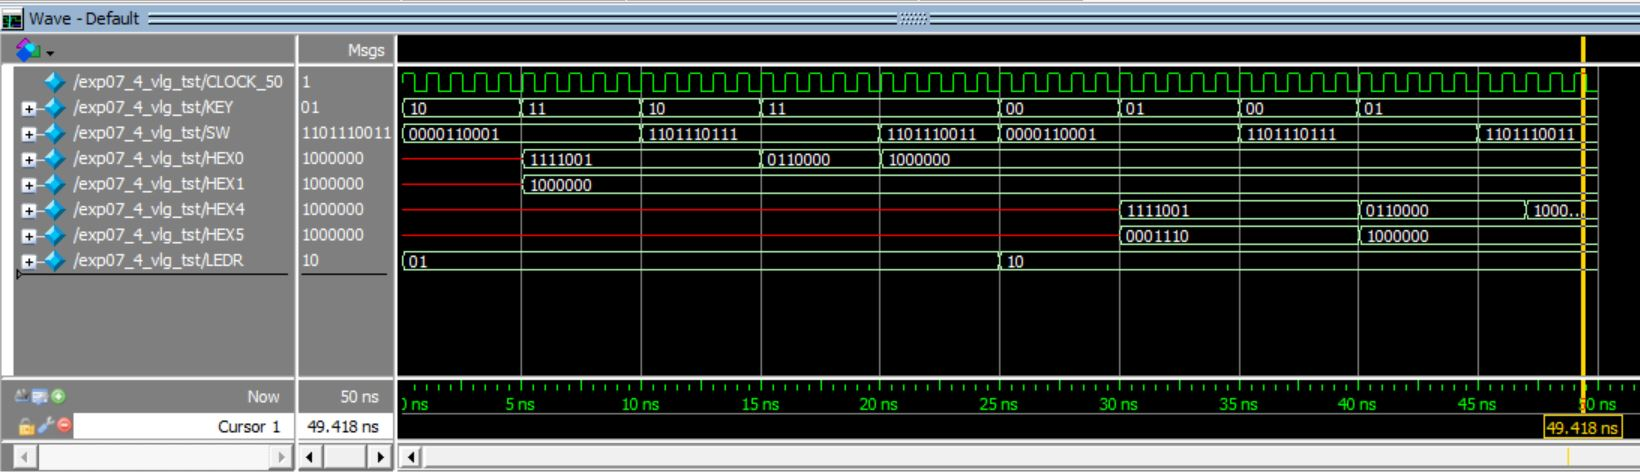
\includegraphics[width=1\textwidth]{sim.JPG}
  \caption{仿真运行结果}
  \label{sim}
\end{figure}

\section{实验结果}
FPGA开发板运行结果展示:

\begin{figure}[H]
  \centering
  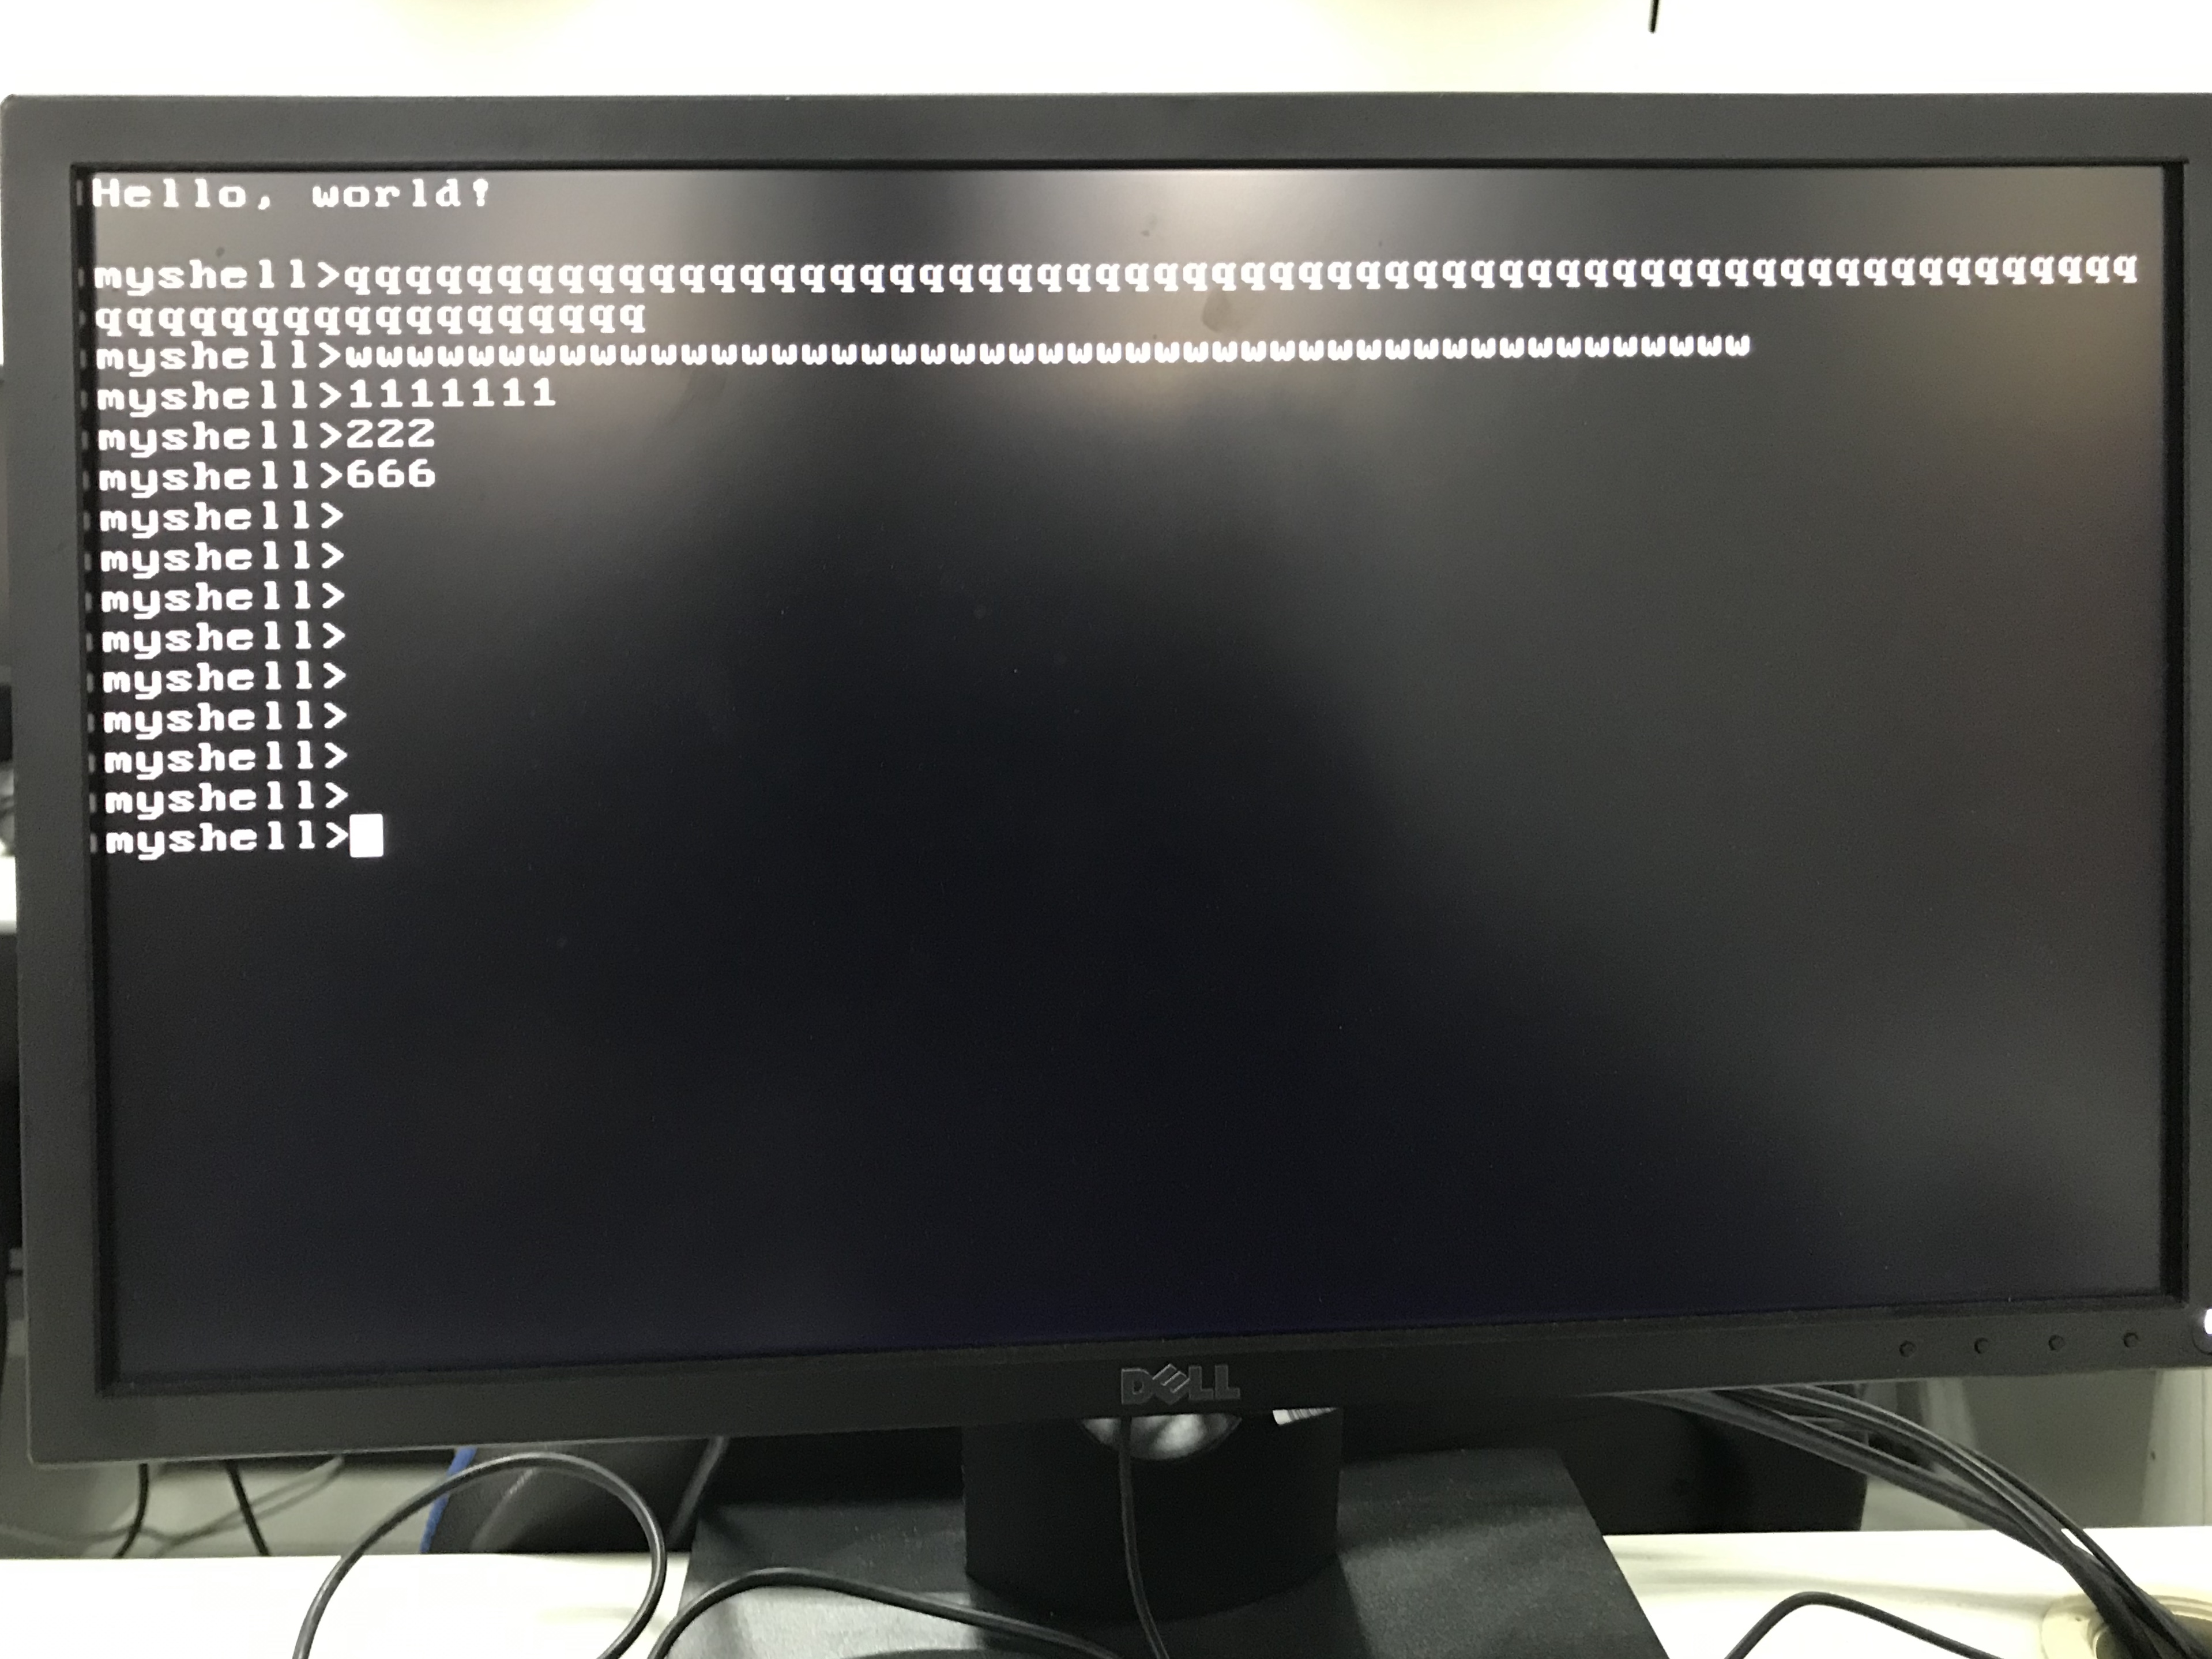
\includegraphics[width=0.8\textwidth]{fpga.JPG}
  \caption{下载运行}
  \label{fpga}
\end{figure}

\section{遇到的问题及解决办法}
\begin{itemize}
  \item 从读取输出地址到七段数码管输出之间至多只能
        有一个非阻塞赋值语句,否则会有延迟
  \item 因为写入的是2位的数据,所以我们最好把写入地址
        对应的8位数据的高6位清零
  \item 用IP核生成的存储器读写数据会有两个系统时钟
        周期的延迟。当输入地址和输出地址相同且
        写使能有效时,记写入之前该地址对应的数据为a,
        写入之后该地址对应的数据为b。如果该存储器的
        输出不受时钟和使能端的控制,那么它会先输出
        一个系统时钟周期的a,此后再输出b。所以需要
        使用非阻塞赋值语句避免输出a
        \begin{figure}[H]
          \centering
          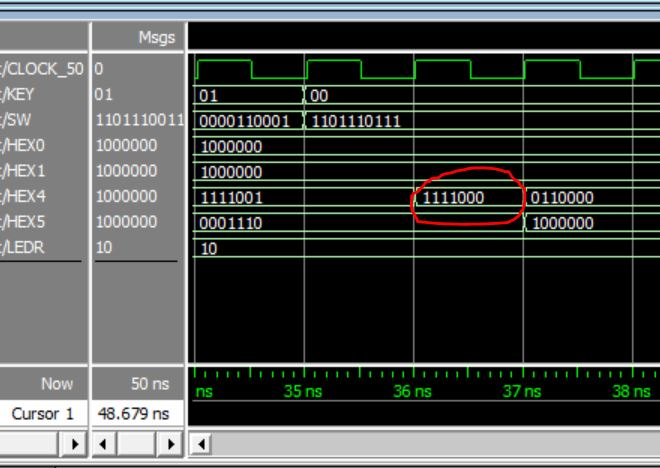
\includegraphics[width=0.8\textwidth]{delay.JPG}
          \caption{输出了应该被覆盖的数据}
          \label{delay}
        \end{figure}
  \item 如果用Switch开关作为存储器使能和写使能的话,
        需要对其进行按键消抖(我也不知道为什么Switch开关
        拨定之后它还是会抖动,明明拨定了却还是会同时读写
        两个存储器,test bench没问题但下载运行就有问题,
        改成用KEY按钮控制使能端就没问题了)
\end{itemize}

\section{得到的启示}
模块化编程能让代码精简不少,但Verilog语言的模块用起来
总感觉有各种说不清的限制。单单是``只能在同一个always
程序块里对同一个变量赋值''就已经很让人头疼了。而且,
为了解决这个问题,就不得不多创建几个中间变量,还需要
尽量少用非阻塞赋值语句对这些变量进行赋值(否则会有很
严重的延迟)。所以比起软件语言而言,Verilog确实
有一些不便之处。

\section{意见和建议}
\begin{itemize}
  \item 意见和建议($\times$)题目纠错($\checkmark$)
  \item 实验7.1的表7-2:RAM代码中,声明ram变量那一行应该是
        \mbox{[RAM\_WIDTH-1:0]}
  \item 实验7.2.1的表7-3:存储器实例代码中,dout0和dout1
        重复声明两遍,可以直接声明为
        \mbox{output reg [7:0] dout0, dout1}
  \item 实验7.3.2对RAM实例化的代码中,应该是``.rdaddress(outaddr)''
\end{itemize}

\end{document}